%  template.tex for Biometrics papers
%
%  This file provides a template for Biometrics authors.  Use this
%  template as the starting point for creating your manuscript document.
%  See the file biomsample.tex for an example of a full-blown manuscript.

%  ALWAYS USE THE referee OPTION WITH PAPERS SUBMITTED TO BIOMETRICS!!!
%  You can see what your paper would look like typeset by removing
%  the referee option.  Because the typeset version will be in two
%  columns, however, some of your equations may be too long. DO NOT
%  use the \longequation option discussed in the user guide!!!  This option
%  is reserved ONLY for equations that are impossible to split across 
%  multiple lines; e.g., a very wide matrix.  Instead, type your equations 
%  so that they stay in one column and are split across several lines, 
%  as are almost all equations in the journal.  Use a recent version of the
%  journal as a guide. 
%  
\documentclass[useAMS, usenatbib, referee]{biom}
%\documentclass[useAMS, usenatbib]{biom}
%
%  If your system does not have the AMS fonts version 2.0 installed, then
%  remove the useAMS option.
%
%  useAMS allows you to obtain upright Greek characters.
%  e.g. \umu, \upi etc.  See the section on "Upright Greek characters" in
%  this guide for further information.
%
%  If you are using AMS 2.0 fonts, bold math letters/symbols are available
%  at a larger range of sizes for NFSS release 1 and 2 (using \boldmath or
%  preferably \bmath).
% 
%  Other options are described in the user guide. Here are a few:
% 
%  -  If you use Patrick Daly's natbib  to cross-reference your 
%     bibliography entries, use the usenatbib option
%
%  -  If you use \includegraphics (graphicx package) for importing graphics
%     into your figures, use the usegraphicx option
% 
%  If you wish to typeset the paper in Times font (if you do not have the
%  PostScript Type 1 Computer Modern fonts you will need to do this to get
%  smoother fonts in a PDF file) then uncomment the next line
%  \usepackage{Times}

%%%%% PLACE YOUR OWN MACROS HERE %%%%%

\def\bSig\mathbf{\Sigma}
\newcommand{\VS}{V\&S}
\newcommand{\tr}{\mbox{tr}}

%  The rotating package allows you to have tables displayed in landscape
%  mode.  The rotating package is NOT included in this distribution, but
%  can be obtained from the CTAN archive.  USE OF LANDSCAPE TABLES IS
%  STRONGLY DISCOURAGED -- create landscape tables only as a last resort if
%  you see no other way to display the information.  If you do do this,
%  then you need the following command.
\usepackage[dvipsnames]{xcolor}
\usepackage{graphicx}
\usepackage[tbtags]{amsmath}

\DeclareMathOperator{\argmax}{arg\,max}
\DeclareMathOperator{\argmin}{arg\,min}
%%%%%%%%%%%%%%%%%%%%%%%%%%%%%%%%%%%%%%%%%%%%%%%%%%%%%%%%%%%%%%%%%%%%%

%  Here, place your title and author information.  Note that in 
%  use of the \author command, you create your own footnotes.  Follow
%  the examples below in creating your author and affiliation information.
%  Also consult a recent issue of the journal for examples of formatting.

\title[Personalized Surveillance Schedules]{Personalized Schedules for Burdensome Surveillance Tests}

%  Here are examples of different configurations of author/affiliation
%  displays.  According to the Biometrics style, in some instances,
%  the convention is to have superscript *, **, etc footnotes to indicate 
%  which of multiple email addresses belong to which author.  In this case,
%  use the \email{ } command to produce the emails in the display.

%  In other cases, such as a single author or two authors from 
%  different institutions, there should be no footnoting.  Here, use
%  the \emailx{ } command instead. 

%  The examples below corrspond to almost every possible configuration
%  of authors and may be used as a guide.  For other configurations, consult
%  a recent issue of the the journal.

%  Single author -- USE \emailx{ } here so that no asterisk footnoting
%  for the email address will be produced.

%\author{John Author\emailx{email@address.edu} \\
%Department of Statistics, University of Warwick, Coventry CV4 7AL, U.K.}

%  Two authors from the same institution, with both emails -- use
%  \email{ } here to produce the asterisk footnoting for each email address

%\author{John Author$^{*}$\email{author@address.edu} and
%Kathy Authoress$^{**}$\email{email2@address.edu} \\
%Department of Statistics, University of Warwick, Coventry CV4 7AL, U.K.}

%  Exactly two authors from different institutions, with both emails  
%  USE \emailx{ } here so that no asterisk footnoting for the email address
%  is produced.

\author{Anirudh Tomer$^{1,*}$\email{a.tomer@erasmusmc.nl}, 
Daan Nieboer$^{2,3}$, 
Monique J. Roobol$^3$, \\
\textbf{Ewout W. Steyerberg}$^{\bmath{4, 2}}$, 
\textbf{and Dimitris Rizopoulos}$^{\bmath{1}}$ \\ \\
$^{1}$Department of Biostatistics, Erasmus University Medical Center, the Netherlands \\
$^{2}$Department of Public Health, Erasmus University Medical Center, the Netherlands \\
$^{3}$Department of Urology, Erasmus University Medical Center, the Netherlands \\
$^{4}$Department of Biomedical Data Sciences, Leiden University Medical Center, the Netherlands}

%  Three or more authors from same institution with all emails displayed
%  and footnoted using asterisks -- use \email{ } 

%\author{John Author$^*$\email{author@address.edu}, 
%Jane Author$^{**}$\email{jane@address.edu}, and 
%Dick Author$^{***}$\email{dick@address.edu} \\
%Department of Statistics, University of Warwick, Coventry CV4 7AL, U.K}

%  Three or more authors from same institution with one corresponding email
%  displayed

%\author{John Author$^*$\email{author@address.edu}, 
%Jane Author, and Dick Author \\
%Department of Statistics, University of Warwick, Coventry CV4 7AL, U.K}

%  Three or more authors, with at least two different institutions,
%  more than one email displayed 

%\author{John Author$^{1,*}$\email{author@address.edu}, 
%Kathy Author$^{2,**}$\email{anotherauthor@address.edu}, and 
%Wilma Flinstone$^{3,***}$\email{wilma@bedrock.edu} \\
%$^{1}$Department of Statistics, University of Warwick, Coventry CV4 7AL, U.K \\
%$^{2}$Department of Biostatistics, University of North Carolina at 
%Chapel Hill, Chapel Hill, North Carolina, U.S.A. \\
%$^{3}$Department of Geology, University of Bedrock, Bedrock, Kansas, U.S.A.}

%  Three or more authors with at least two different institutions and only
%  one email displayed

%\author{John Author$^{1,*}$\email{author@address.edu}, 
%Wilma Flinstone$^{2}$, and Barney Rubble$^{2}$ \\
%$^{1}$Department of Statistics, University of Warwick, Coventry CV4 7AL, U.K \\
%$^{2}$Department of Geology, University of Bedrock, Bedrock, Kansas, U.S.A.}
\begin{document}

%  This will produce the submission and review information that appears
%  right after the reference section.  Of course, it will be unknown when
%  you submit your paper, so you can either leave this out or put in 
%  sample dates (these will have no effect on the fate of your paper in the
%  review process!)

\date{{\it Received October} 0000. {\it Revised February} 0000.  {\it
Accepted March} 0000.}

%  These options will count the number of pages and provide volume
%  and date information in the upper left hand corner of the top of the 
%  first page as in published papers.  The \pagerange command will only
%  work if you place the command \label{firstpage} near the beginning
%  of the document and \label{lastpage} at the end of the document, as we
%  have done in this template.

%  Again, putting a volume number and date is for your own amusement and
%  has no bearing on what actually happens to your paper!  

\pagerange{\pageref{firstpage}--\pageref{lastpage}} 
\volume{00}
\pubyear{0000}
\artmonth{December}

%  The \doi command is where the DOI for your paper would be placed should it
%  be published.  Again, if you make one up and stick it here, it means 
%  nothing!

\doi{10.1111/j.1541-0420.2005.00454.x}

%  This label and the label ``lastpage'' are used by the \pagerange
%  command above to give the page range for the article.  You may have 
%  to process the document twice to get this to match up with what you 
%  expect.  When using the referee option, this will not count the pages
%  with tables and figures.  

\label{firstpage}

%  put the summary for your paper here

% !TEX root =  ../main_manuscript.tex 
\begin{abstract}
\texttt{Background}: Prostate cancer active surveillance (AS) patients undergo repeat biopsies. Active treatment is advised when biopsy Gleason grade group~$\geq$~2 (\textit{upgrading}). Many patients never experience upgrading, yet undergo biopsies frequently. Personalized biopsy decisions based on upgrading-risk may reduce patient burden.\\

\texttt{Objective}: Develop a risk prediction model and web-application to assist patients/doctors in personalized biopsy decisions.\\

\texttt{Design, Setting, and Participants}: Model development: world's largest AS study PRIAS, 7813 patients, 1134 experienced upgrading; External validation: largest five cohorts of Movember Foundation's GAP3 database (${>20,000}$ patients, 27 centers worldwide); Data: repeat prostate-specific antigen (PSA) and biopsy Gleason grade.\\

\texttt{Outcome Measurements, and Statistical Analysis}: A Bayesian joint model fitted to the PRIAS dataset. This model was validated in GAP3 cohorts using risk prediction error, calibration, area under ROC (AUC). Model and personalized biopsy schedules based on predicted risks were implemented in a web-application.\\

\texttt{Results and Limitations}: Cause-specific cumulative upgrading-risk at year five of follow-up: 35\% in PRIAS, at most 50\% in GAP3 cohorts. PRIAS based model: PSA velocity was a stronger predictor of upgrading (Hazard~Ratio:~2.47, 95\%CI:~1.93--2.99) than PSA value (Hazard~Ratio:~0.99, 95\%CI:~0.89--1.11). Validation: Moderate AUC (0.55--0.75) in PRIAS and GAP3 cohorts. Moderate prediction error (0.1--0.3) in GAP3 cohorts where impact of PSA value and velocity on upgrading-risk was similar to PRIAS, but large (0.3--0.45) otherwise. Recalibration advised for external cohorts.\\

\texttt{Conclusions}: We successfully developed and validated a model for predicting upgrading-risk, and providing risk-based personalized biopsy decisions, in prostate cancer AS. The model made available via a web-application enables shared decision making of biopsy schedules by comparing fixed and personalized schedules on total biopsies and expected time delay in detecting upgrading.\\

\texttt{Patient Summary}: Personalized prostate biopsies are a novel alternative to fixed one-size-fits-all schedules. The underlying statistical models are made available through a user-friendly web-application and may help to reduce unnecessary prostate biopsies while maintaining cancer control.
\end{abstract}

%  Please place your key words in alphabetical order, separated
%  by semicolons, with the first letter of the first word capitalized,
%  and a period at the end of the list.
%
\begin{keywords}
Chronic NCDs; Invasive diagnostic tests; Joint models; Personalized schedules; Prostate biopsy; Surveillance
\end{keywords}

%  As usual, the \maketitle command creates the title and author/affiliations
%  display 

\maketitle

%  If you are using the referee option, a new page, numbered page 1, will
%  start after the summary and keywords.  The page numbers thus count the
%  number of pages of your manuscript in the preferred submission style.
%  Remember, ``Normally, regular papers exceeding 25 pages and Reader Reaction 
%  papers exceeding 12 pages in (the preferred style) will be returned to 
%  the authors without review. The page limit includes acknowledgements, 
%  references, and appendices, but not tables and figures. The page count does 
%  not include the title page and abstract. A maximum of six (6) tables or 
%  figures combined is often required.''

%  You may now place the substance of your manuscript here.  Please use
%  the \section, \subsection, etc commands as described in the user guide.
%  Please use \label and \ref commands to cross-reference sections, equations,
%  tables, figures, etc.
%
%  Please DO NOT attempt to reformat the style of equation numbering!
%  For that matter, please do not attempt to redefine anything!

% !TEX root =  ../main_manuscript.tex 
\section{Introduction}
Patients with low- and very low-risk screening-detected localized prostate cancer are usually advised active surveillance (AS) instead of immediate radical treatment~\citep{briganti2018active}. In AS, cancer progression is routinely monitored via prostate-specific antigen (PSA), digital rectal examination, and repeat biopsies. Among these, the strongest indicator of cancer-related outcomes is the biopsy Gleason grade~\citep{epsteinGG2014}. When the Gleason grade increases from grade~1 (Gleason 3+3) to 2 (Gleason 3+4) or higher, called \textit{reclassification}, patients are commonly advised curative treatment~\citep{bul2013active}.

\begin{figure}
\centerline{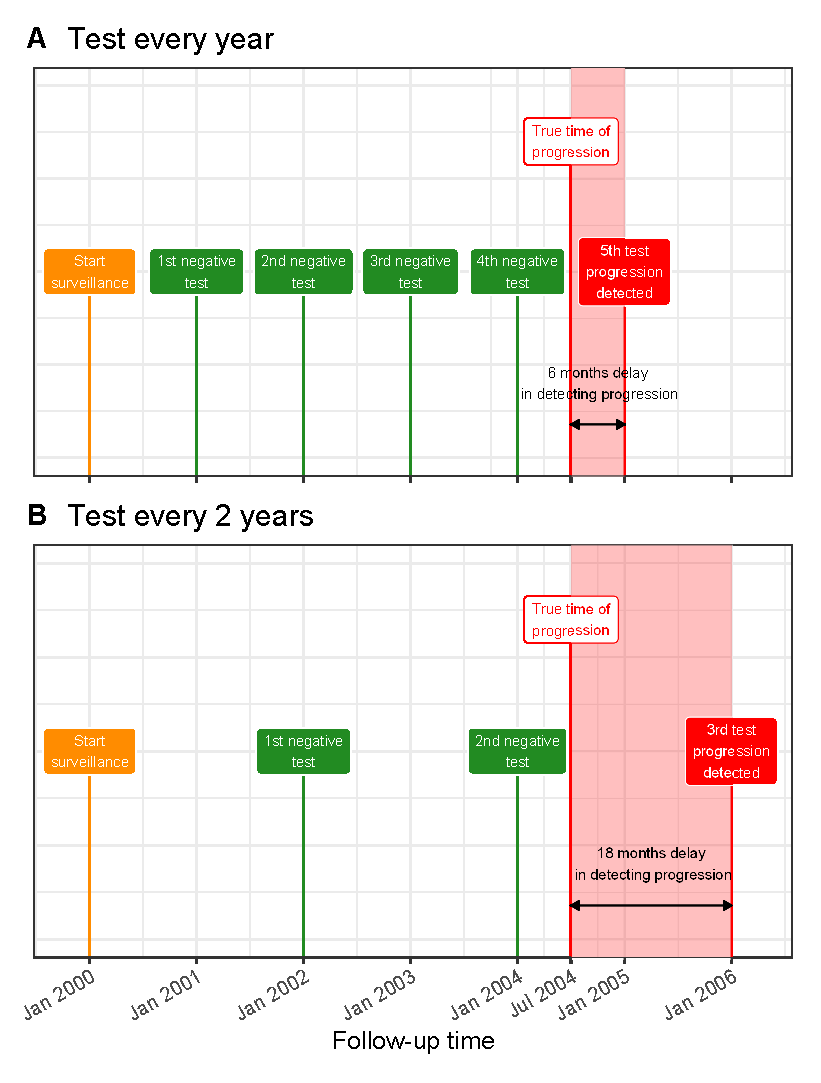
\includegraphics[width=\columnwidth]{images/delay_explanation.eps}}
\caption{\textbf{Trade-off between the number of biopsies and time delay in detecting reclassification (Increase in Gleason grade from 1 to 2 or higher):} The true time of reclassification for the patient in this figure is July 2008. When biopsies are scheduled annually (\textbf{Panel~A}), reclassification is detected in January 2009 with a time delay of six months, and a total of four biopsies are scheduled. When biopsies are scheduled biennially (\textbf{Panel~B}) reclassification is detected in January 2010 with a time delay of 18 months, and a total of three biopsies are scheduled. Since biopsies are conducted periodically, the time of reclassification is observed as an interval. For example, between Jan~2008--Jan~2009 in \textbf{Panel~A} and between Jan~2008--Jan~2010 in \textbf{Panel~B}.}
\label{fig:delay_explanation}
\end{figure}

Biopsies are conducted periodically. Consequently, reclassification is always detected with a time delay (Figure~\ref{fig:delay_explanation}). For detecting reclassification timely, many AS programs schedule fixed and frequent biopsies (e.g.,~annually) for all patients~\citep{nieboer2018active,loeb2014heterogeneity}. However, this also leads to many unnecessary biopsies in slow/non-progressing patients. Biopsies are invasive, painful and prone to medical complications. Thus, biopsy burden and patient non-compliance to frequent biopsies~\citep{bokhorst2015compliance} has raised concerns regarding the optimal biopsy schedule~\citep{inoue2018comparative, bratt2013study}. To this end, infrequent schedules such as biennial biopsies have been proposed as an alternative~\citep{inoue2018comparative,de2017estimating}. Although, biennial biopsies may still lead to five unnecessary biopsies over ten years (current study period of large AS programs) for slow/non-progressing patients. A promising alternative to fixed and frequent biopsies is personalized biopsy schedules based on the patient-specific risk of reclassification (Figure~\ref{fig:riskBasedExample}).

\begin{figure}
\centerline{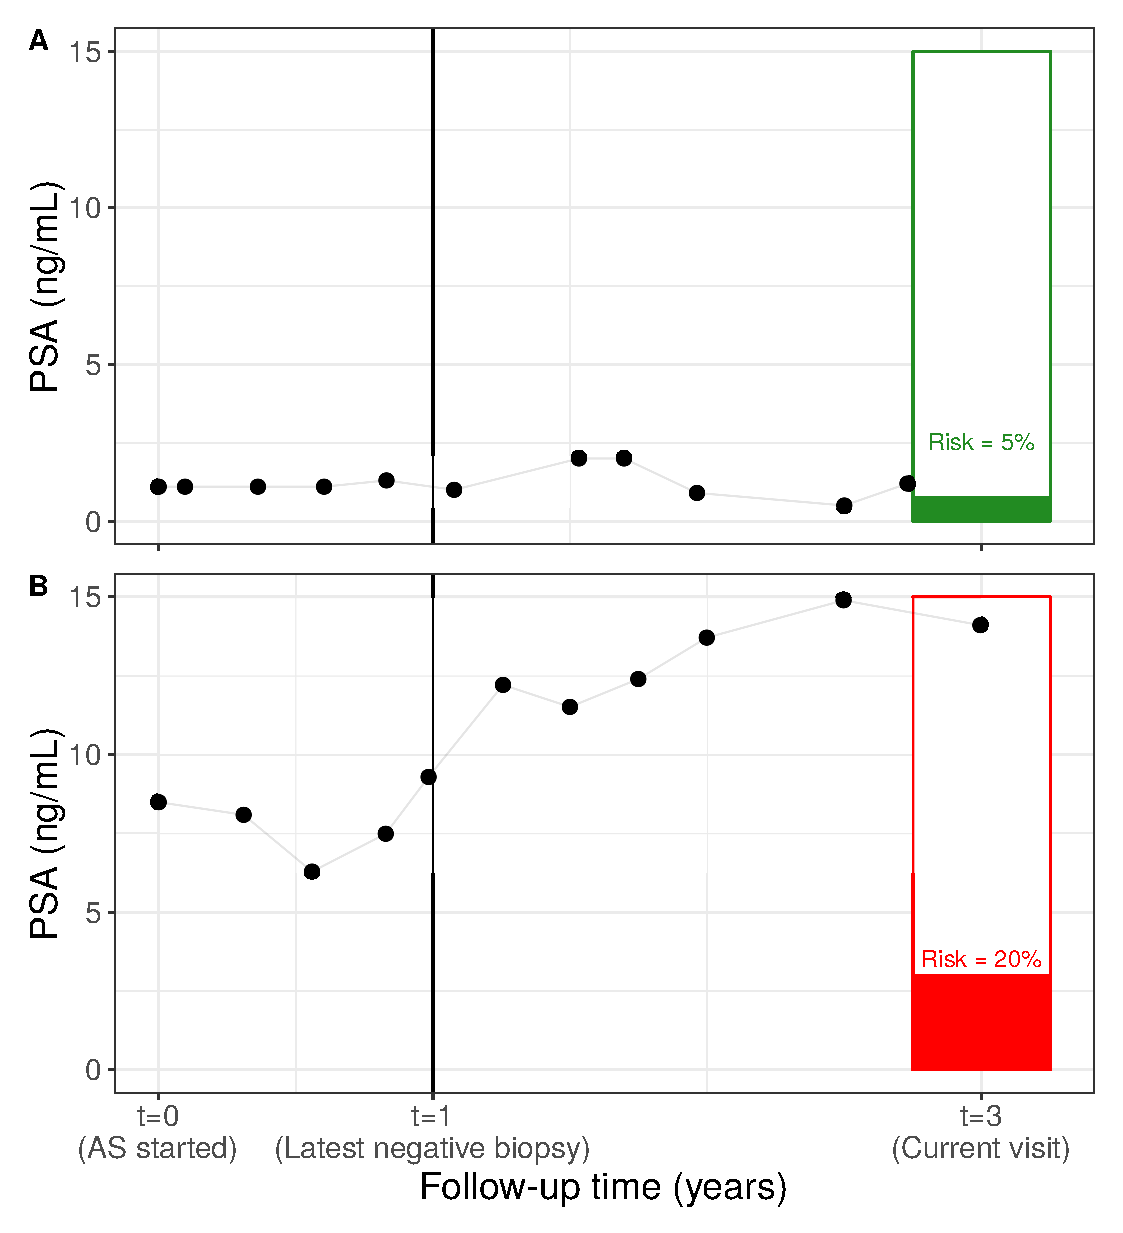
\includegraphics[width=\columnwidth]{images/riskBasedExample.eps}}
\caption{\textbf{Motivation for personalized risk-based decisions of biopsy}: Patient~A (\textbf{Panel~A}) and B (\textbf{Panel~B}) had their latest biopsy at year one of follow-up (green vertical line). Patient~A's prostate-specific antigen (PSA) profile remained stable until his current visit at year three, whereas patient~B's profile has shown a rise. Consequently, patient~B's estimated cumulative risk of reclassification at the current visit (year three) is higher than that of patient~A. This makes patient~B a more suitable candidate for biopsy than Patient~A. Risk estimates in this figure are only illustrative.}
\label{fig:riskBasedExample}
\end{figure}

The first challenge in developing personalized biopsy schedules is consolidating accumulated patient data (e.g., PSA, previous biopsy results) into risk estimates for reclassification. Existing calculators for risk of reclassification~\citep{partin1993use,makarov2007updated} use only the latest PSA measurement of a patient. In contrast, we intend to utilize all repeated measurements of PSA, previous biopsy results, and baseline characteristics of a patient. To this end, a suitable model is the joint model for time-to-event and longitudinal data~\citep{tomer2019, coley2017prediction,rizopoulos2012joint}. A joint model predicts risk of reclassification in a personalized manner. A subsequent challenge however, is translating risks into clinical decisions. For example, a 10\% risk of reclassification can be perceived high/low depending upon the patient age. Patients may also weigh risks of reclassification with the potential \textit{consequences} of another biopsy. Two relevant \textit{consequences} of biopsies (Figure~\ref{fig:delay_explanation}) are the timing and total number of biopsies (burden), and the time delay in detecting reclassification (smaller is beneficial). The relative importance of these \textit{consequences} can vary between the patients, and also over the follow-up period for the same patient.

The goal of this work was to assist patients and doctors in making better decisions of biopsies than fixed and frequent biopsies. For this purpose, we developed a web-application that gives patients their current and future risk of reclassification. It also suggests them risk-based personalized schedules of biopsies. For each biopsy schedule, be it fixed or personalized, the web-application provides expected \textit{consequences} of following it. Thus, patients can compare schedules before making a decision. The web-application uses a prediction joint model fitted to the world's largest AS dataset, PRIAS~\citep{bul2013active}. We externally validated this model in five largest AS cohorts of the GAP3 database \citep{gap3_2018}. Thus, the web-application can be used by a large number of patients worldwide.
% !TEX root =  ../main_manuscript.tex 
\section{Joint Model for Time-to-Progression and Longitudinal Outcomes}
\label{sec:jointmodel}
Let $T_i^*$ denote the true time of disease progression for the ${i\mbox{-th}}$ patient. Progression is always interval censored ${l_i < T_i^* \leq r_i}$ (Figure~\ref{fig:delay_explanation}). Here, $r_i$ and $l_i$ denote the time of the last and second last invasive tests, respectively, when patients progress. In non-progressing patients, $l_i$ denotes the time of the last test and ${r_i=\infty}$. Assuming $K$ types of longitudinal outcomes, let $\boldsymbol{y}_{ki}$ denote the ${n_{ki} \times 1}$ longitudinal response vector of the ${k\mbox{-th}}$ outcome, $k \in \{1, \ldots, K\}$. The observed data of all $n$ patients is given by ${\mathcal{A}_n = \{l_i, r_i, \boldsymbol{y}_{1i},\ldots \boldsymbol{y}_{Ki}; i = 1, \ldots, n\}}$.

\subsection{Longitudinal Sub-process}
To model multiple longitudinal outcomes in a unified framework, a joint model employs individual generalized linear mixed sub-models~\citep{mcculloch2005generalized}. Specifically, the conditional distribution of the $k$-th outcome $\boldsymbol{y}_{ki}$ given a vector of patient-specific random effects $\boldsymbol{b}_{ki}$ is assumed to belong to the exponential family, with linear predictor given by,
\begin{equation*}
\label{eq:long_model}
g_k\big[E\{y_{ki} (t) \mid \boldsymbol{b}_{ki}\}\big] = m_{ki}(t) = \boldsymbol{x}_{ki}^{\top}(t)\boldsymbol{\beta}_{k} + \boldsymbol{z}_{ki}^{\top}(t)\boldsymbol{b}_{ki},
\end{equation*}
where $g_k(\cdot)$ denotes a known one-to-one monotonic link function, $y_{ki}(t)$ is the
value of the ${k\mbox{-th}}$ longitudinal outcome for the ${i\mbox{-th}}$ patient at time $t$, and $\boldsymbol{x}_{ki}(t)$ and $\boldsymbol{z}_{ki}(t)$ are the time-dependent design vectors for the fixed $\boldsymbol{\beta}_{k}$ and random effects $\boldsymbol{b}_{ki}$, respectively. To model the correlation between different longitudinal outcomes, we link their corresponding random effects. Specifically, we assume that the vector of random effects ${\boldsymbol{b}_{i} = (\boldsymbol{b}_{1i}^{\top}, \ldots, \boldsymbol{b}_{Ki}^{\top})^{\top}}$ follows a multivariate normal distribution with mean zero and variance-covariance matrix $W$.

\subsection{Survival Sub-process}
\label{subsec:surival_sub_model}
In the survival sub-process, the hazard of progression $h_i(t)$ at a time $t$ is assumed to depend on a function of patient and outcome-specific linear predictors $m_{ki}(t)$ and/or the random effects,
\begin{equation*}
\label{eq:rel_risk_model}
h_i\big\{t \mid \mathcal{M}_i(t), \boldsymbol{w}_i(t)\big\} = h_0(t) \exp\Big[\boldsymbol{\gamma}^{\top}\boldsymbol{w}_i(t) + \sum_{k=1}^{K} f_{k} \big\{ \mathcal{M}_{ki}(t), \boldsymbol{w}_i(t), \boldsymbol{b}_{ki}, \boldsymbol{\alpha}_{k} \big\}\Big], \quad t>0,
\end{equation*}
where $h_0(\cdot)$ denotes the baseline hazard, $\mathcal{M}_{ki}(t)=\{m_{ki}(s) \mid 0 \leq s < t \}$ is the history of the ${k\mbox{-th}}$ longitudinal process up to $t$, and $\boldsymbol{w}_i(t)$ is a vector of exogenous, possibly time-varying covariates with regression coefficients $\boldsymbol{\gamma}$. Functions $f_{k}(\cdot)$, parameterized by vector of coefficients $\boldsymbol{\alpha_{k}}$, specify the features of each longitudinal outcome that are included in the linear predictor of the relative-risk model~\citep{brown2009assessing,rizopoulos2012joint,taylor2013real}. Some examples, motivated by the literature (subscripts $k$ dropped for brevity), are,
\begin{eqnarray*}
\left \{
\begin{array}{l}
f\big\{\mathcal{M}_{i}(t), \boldsymbol{w}_i(t), \boldsymbol{b}_{i}, \boldsymbol{\alpha} \big\} = \alpha m_{i}(t),\\
f\big\{ \mathcal{M}_{i}(t), \boldsymbol{w}_i(t), \boldsymbol{b}_{i}, \boldsymbol{\alpha}\big\} = \alpha_1 m_{i}(t) + \alpha_2 m'_{i}(t),\quad \text{with}\  m'_{i}(t) = \frac{\mathrm{d}{m_{i}(t)}}{\mathrm{d}{t}}.\\
\end{array}
\right.
\end{eqnarray*}
These formulations of $f(\cdot)$ postulate that the hazard of progression at time $t$ may depend on the underlying level $m_i(t)$ (e.g., PSA value in prostate cancer) or on both the level and velocity $m'_i(t)$ (e.g., PSA velocity) of the longitudinal outcome at $t$. Lastly, the baseline hazard $h_0(t)$ is modeled flexibly using P-splines~\citep{eilers1996flexible}. The detailed specification of the baseline hazard, and the joint parameter estimation of the longitudinal and relative-risk sub-models using the Bayesian approach are presented in Supplementary~A.
% !TEX root =  ../main_manuscript.tex 
\section{Personalized Schedule of Invasive Tests for Detecting Progression}
\label{sec:schedule}
We intend to develop a personalized schedule of invasive tests for a new patient $j$, not present in training dataset $\mathcal{A}_n$. Tests are conducted only until progression is detected (Figure~\ref{fig:delay_explanation}). Let $T^*_j$ be the true time of progression, and ${t < T^*_j}$ be the time of the last conducted test on which progression was not detected for the $j$-th patient. Lastly, ${v > t}$ denotes the time of the current follow-up visit.

\subsection{Cumulative-risk of progression}
\label{subsec:cum_risk}
First we combine the history of observed longitudinal outcomes $\{\mathcal{Y}_{1j}(v), \ldots, \mathcal{Y}_{Kj}(v)\}$ until the current visit time $v$, and the result of the last conducted test ${T^*_j > t}$ to define the patient-specific cumulative-risk of progression at future time $u$ (Figure~\ref{fig:dynrisk_explanation}).
\begin{equation}
\label{eq:cumulative_risk}
\begin{split}
R_j(u \mid t, v) &= \mbox{Pr}\big\{T^*_j \leq u \mid T^*_j > t, \mathcal{Y}_{1j}(v), \ldots, \mathcal{Y}_{Kj}(v), \mathcal{A}_n\big\}\\
&=\int \int \mbox{Pr}(T^*_j \leq u \mid T^*_j > t, \boldsymbol{b}_{j}, \boldsymbol{\theta}) p\big\{\boldsymbol{b}_j \mid T^*_j > t, \mathcal{Y}_{1j}(v), \ldots, \mathcal{Y}_{Kj}(v), \boldsymbol{\theta} \big\}\\
&\quad \times p(\boldsymbol{\theta} \mid \mathcal{A}_n) \mathrm{d}\boldsymbol{b}_j \mathrm{d}\boldsymbol{\theta}, \quad u \geq t.
\end{split}
\end{equation}
The personalized cumulative-risk function $R_j(\cdot)$ depends on the observed longitudinal data $\{\mathcal{Y}_{1j}(v), \ldots, \mathcal{Y}_{Kj}(v)\}$, and the training dataset $\mathcal{A}_n$ via the posterior distribution of patient-specific random effects~$\boldsymbol{b}_j$, and posterior distribution of the vector of joint model parameters~$\boldsymbol{\theta}$, respectively. The risk also dynamically updates as more longitudinal data becomes available over follow-up (Panel~B~and~C, Figure~\ref{fig:dynrisk_explanation}).

\begin{figure}
\centerline{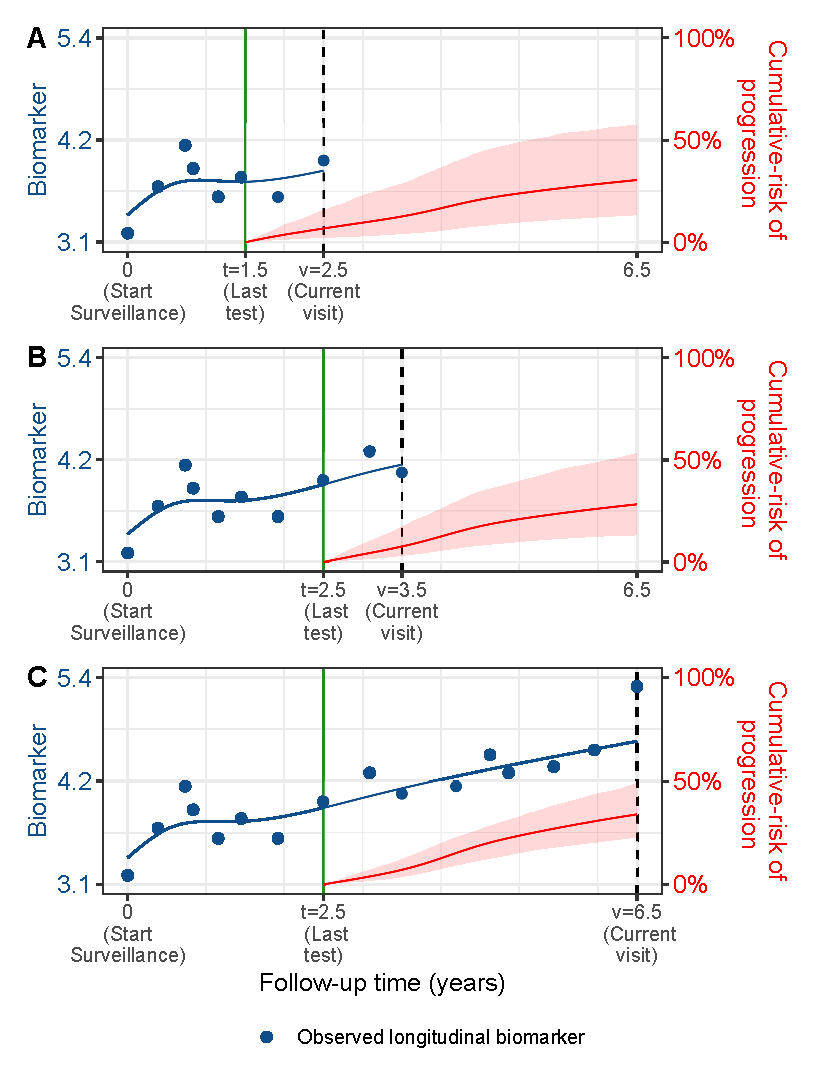
\includegraphics{images/dynrisk_plot_102.eps}}
\caption{\textbf{Cumulative-risk of progression changing dynamically over follow-up} as more patient data is gathered. A single longitudinal outcome, namely, a continuous biomarker of disease progression, is used for illustration. \textbf{Panels~A,~B~and~C:} are ordered by the time of the current visit (dashed vertical black line) of a new patient. At each of these visits, we combine the accumulated longitudinal measurements (shown in blue), and last time of negative invasive test (solid vertical green line) to obtain the updated cumulative-risk profile (shown in red) of the patient. All values are illustrative.} 
\label{fig:dynrisk_explanation}
\end{figure}

\subsection{Personalized Schedule of Tests Using a Cumulative-risk Threshold $\kappa^*$}
\label{subsec:pers_schedule}
Our aim is to employ the cumulative-risk function in~(\ref{eq:cumulative_risk}) to develop a risk-based personalized schedule of invasive tests for the $j$-th patient. Typically an invasive test is decided on the same visit on which auxiliary data (e.g., biomarkers) is measured. Let $U={u_1, \ldots, u_L}$ represent a schedule of such visits (e.g., every six months in prostate cancer for PSA measurement), where $u_1=v$ is also the time of the current visit.

First, we make $L$ successive decisions for conducting tests on each of the $L$ future visit times $u_l \in U$. Specifically, we decide to conduct a test at time $u_l$ if the conditional cumulative-risk of progression at $u_l$ is larger than a certain risk threshold $0 \leq \kappa^* \leq 1$ (e.g., $\kappa^*=10$\% risk). If a test gets planned at time $u_l$, then the successive test decision at time $u_{l+1}$ is made using an updated cumulative-risk profile (Figure~\ref{fig:schedule_explanation}). This updated cumulative-risk profile accounts for the possibility that progression may occur after time $u_l < T^*_j$. The test decisions on each future visit time $u_l$ are defined as:
\begin{equation*}
\label{eq:personalized_decision_grid}
\begin{split}
Q_j^{\kappa^*}(u_l \mid t_l, v) &= I\big\{R_j(u_l \mid t_l, v) \geq \kappa^* \big\},\\
t_l &= \left\{\begin{array}{lcr}
  t, &\mbox{if}& l=1\\
  t_{l-1}, &\mbox{if}&  Q_j^{\kappa^*}(u_{l-1} \mid t_{l-1}, v)=0, l\geq 2\\ 
  u_{l-1}, &\mbox{if}&  Q_j^{\kappa^*}(u_{l-1} \mid t_{l-1}, v)=1, l\geq 2\\
\end{array} \right\}.
\end{split}
\end{equation*}
The cumulative-risk $R_j(u_l \mid t_l, v)$ at future visit time $u_l$ utilizes the time $t_l$ as the time of the last conducted test on which progression may not be observed~(\ref{eq:cumulative_risk}). However, the contribution of the observed longitudinal data $\{\mathcal{Y}_{1j}(v), \ldots, \mathcal{Y}_{Kj}(v)\}$ in the risk function remains the same over all time points in $U$. The test decision at time $u_l$ is denoted by ${Q_j^{\kappa^*}(u_l \mid t_l, v)}$. Via the indicator function $I(\cdot)$ it obtains a value 1 (or 0) when a test is to be conducted (or not conducted) at time $u_l$. The subset of future time points in $U$ on which a test is to be performed results into a personalized schedule of planned future tests, given by:
\begin{equation}
\label{eq:personalized_schedule_grid}
S_j^{\kappa^*}(U \mid t, v) = \big\{ u_l \in U \mid Q_j^{\kappa^*}(u_l \mid t_l, v)=1\big\}.
\end{equation}
The personalized schedule in~(\ref{eq:personalized_schedule_grid}) is updated as more patient data becomes available over subsequent follow-up visits.

\begin{figure}
\centerline{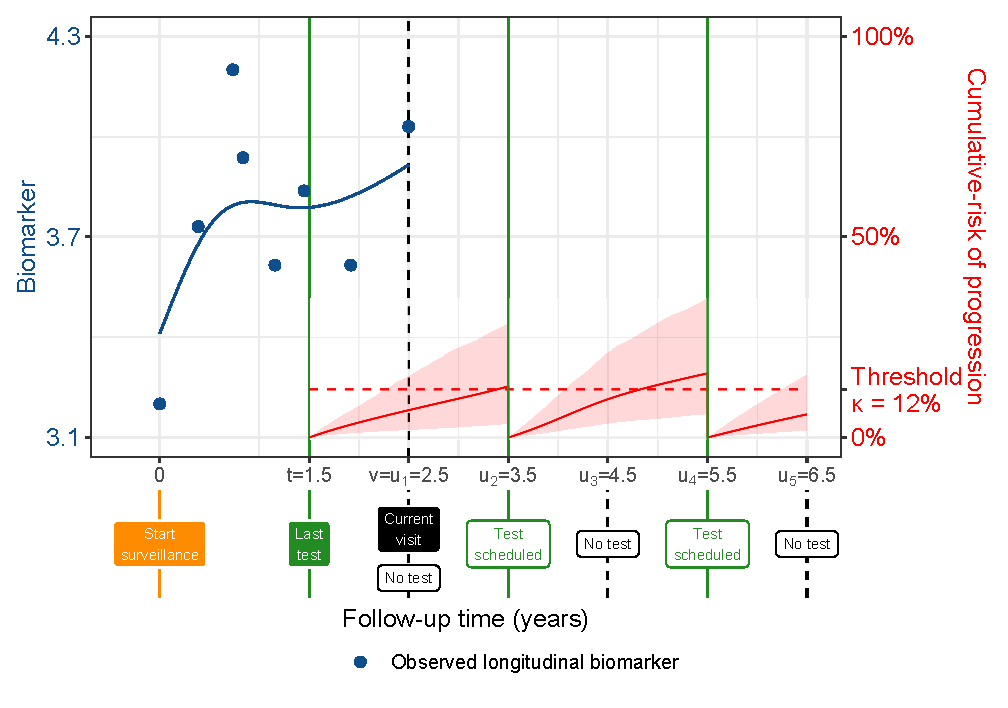
\includegraphics{images/schedule_explanation_102.eps}}
\caption{\textbf{Personalized Invasive Test Schedule Using Patient-specific Conditional Cumulative-risk of Progression}.  A single longitudinal outcome, namely, a continuous biomarker (observed: blue dots, fitted: blue line) of disease progression is used for illustration. The last test on which progression was not observed was conducted at $t=1.5$ years. The current visit time of the patient is $v=2.5$ years. Decisions for invasive test need to be made at a gap of every one year starting from the current visit until a horizon of 6.5 years. That is, $U=\{2.5, 3.5, 4.5, 5.5, 6.5\}$ years. Based on an example risk threshold of 12\% ($\kappa^*=0.12$) the future test decisions at time points in $U$ lead to a personalized schedule $S_j^{\kappa^*} (U \mid t=1.5, v=2.5) = \{3.5, 5.5\}$ years. The conditional cumulative-risk profiles $R_j(u_l \mid t_l, v)$ employed in~(\ref{eq:personalized_decision_grid}) are shown with red line (confidence interval shaded). It is called `conditional' because, for example, the second test at future time 5.5 years, is scheduled after accounting for the possibility that progression (true time $T^*_j$) may not have occurred until the time of the previously scheduled test at time $T^*_j>3.5$ years. All values are illustrative.} 
\label{fig:schedule_explanation}
\end{figure}

\subsection{Expected Number of Tests and Time Delay in Detecting Progression}
\label{subsec:exp_delay_estimation}
The schedule $S_j^{\kappa^*}(U \mid t, v)$ manifests a personalized test plan for the $j$-the patient. However, the number of tests that will get conducted and the time delay in detecting progression that may subsequently be observed (Figure~\ref{fig:delay_explanation}), depends on the true time of progression $T^*_j$ of the patient. Since two different patients with the same timing of tests will expect different number of tests and time delay, we estimate these two quantities in a patient-specific manner as well. Although, this calculation is not limited to personalized schedules only, but can be done for any schedule of tests. More specifically, given a schedule $S$ with tests planned at $S=\{s_n \mid n=1,\ldots, N\}$, we calculate the expected number of tests and delay for the scenario that the patient obtains progression before the time of the last test $T^*_j \leq s_N$.

If $T^*_j \leq s_N$ then for each of the $N$ test times $s_n \in S$ there exist $N$ time intervals ${s_{n-1} < T^*_j \leq s_n}$ in which progression may be observed. Correspondingly, there are $N$ possible number of tests $(1,\ldots, N)$, and $N$ possible time delays $s_n - T^*_j$ in detecting progression. Specifically, the true number of tests $N_j$ and true time delay in detecting progression $D_j$ that the patient will experience can be defined as:
\begin{equation}
\label{eq:number_of_tests_and_delay}
\begin{split}
N_j (S \mid t) &= \left\{ \begin{array}{lcr}
  1, &\mbox{if}& t < T^*_j \leq s_1\\
  \ldots \\
  N, &\mbox{if}& s_{N-1} < T^*_j \leq s_{N}  
\end{array} \right\},\\
D_j (S \mid t) &= \left\{ \begin{array}{lcrr}
  s_1 - T^*_j, &\mbox{if}& t < T^*_j \leq s_1\\
  \ldots \\
  s_N - T^*_j, &\mbox{if}& s_{N-1} < T^*_j \leq s_N  
\end{array} \right\}.
\end{split}
\end{equation}
To estimate the expected values of both $N_j(\cdot)$ and $D_j(\cdot)$ in a patient-specific manner, we exploit the personalized cumulative-risk profile of the patient defined in~(\ref{eq:cumulative_risk}). Specifically, the expected number of tests $E\{N_j(\cdot)\}$ and expected time delay $E\{D_j(\cdot)\}$ can be calculated as the weighted sum of $N$ possible number of tests and time delays defined in~(\ref{eq:number_of_tests_and_delay}). The $n$-th weight is equal to the probability $\mbox{Pr}(s_{n-1} < T^*_j \leq s_n \mid T^*_j \leq s_N)$ of the patient obtaining progression in the $n$-th interval ${s_{n-1} < T^*_j \leq s_n}$.
%\begin{equation}
%\label{eq:expected_number_of_tests_and_delay}
%\begin{split}
%E\big\{N_j(S \mid t)\big\} &= \sum_{n=1}^{N-1} n \times \mbox{Pr}(s_{n-1} < T^*_j \leq s_n) + N \times \mbox{Pr}(T^*_j > s_{N-1}), \quad s_0 = t\\
%E\big\{D_j(S \mid t)\big\} &= \sum_{n=1}^{N} \Big\{s_n - E(T^*_j \mid s_{n-1}, s_n, v)\Big\} \times \mbox{Pr}(s_{n-1} < T^*_j \leq s_n) , \quad s_0 = t\\
%E(T^*_j \mid s_{n-1}, s_n, v) &= s_{n-1} + \int_{s_{n-1}}^{s_n} \mbox{Pr}\Big\{T^*_j \geq u \mid s_{n-1} < T^*_j \leq s_n, \mathcal{Y}_{1j}(v), \ldots, \mathcal{Y}_{Kj}(v), \mathcal{A}_n\Big\} \mathrm{d}u\\
%\mbox{Pr}(s_{n-1} < T^*_j \leq s_n) &= R_j(s_n \mid t, v) - R_j(s_{n-1} \mid t, v)\\
%\mbox{Pr}(T^*_j > s_{N-1}) &= 1- R_j(s_{N-1} \mid t, v),
%\end{split}
%\end{equation}
\begin{equation*}
\label{eq:expected_number_of_tests_and_delay}
\begin{split}
E\big\{N_j(S \mid t)\big\} &= \sum_{n=1}^{N-1} n \times \mbox{Pr}(s_{n-1} < T^*_j \leq s_n \mid T^*_j \leq s_N), \quad s_0 = t\\
E\big\{D_j(S \mid t)\big\} &= \sum_{n=1}^{N} \Big\{s_n - E(T^*_j \mid s_{n-1}, s_n, v)\Big\} \times \mbox{Pr}(s_{n-1} < T^*_j \leq s_n\mid T^*_j \leq s_N)\\
E(T^*_j \mid s_{n-1}, s_n, v) &= s_{n-1} + \int_{s_{n-1}}^{s_n} \mbox{Pr}\Big\{T^*_j \geq u \mid s_{n-1} < T^*_j \leq s_n, \mathcal{Y}_{1j}(v), \ldots, \mathcal{Y}_{Kj}(v), \mathcal{A}_n\Big\} \mathrm{d}u\\
\mbox{Pr}(s_{n-1} < T^*_j \leq s_n\mid T^*_j \leq s_N) &= \frac{R_j(s_n \mid t, v) - R_j(s_{n-1} \mid t, v)}{R_j(s_N \mid t, v)},
\end{split}
\end{equation*}
where $E(T^*_j \mid s_{n-1}, s_n, v)$ denotes the conditional expected time of progression for the scenario $s_{n-1} < T^*_j \leq s_n$, and is calculated as the area under the corresponding survival curve.

The personalized expected number of tests and expected time delay in detecting progression have the advantage that they are updated over follow-up as more patient data becomes available. Since they can be calculated for any schedule, patients and doctors can utilize them to compare schedules before making a decision. Although, in order to have a fair comparison of time delays between different schedules for the same patient, a compulsory test at a common horizon time point should be planned in all schedules.

\subsection{Choice of Risk Threshold $\kappa^*$}
The risk threshold $\kappa^*$ controls the timing and the total number of invasive tests in the personalized schedule $S_j^{\kappa^*}(U \mid t, v)$. Through the timing and the total number of planned tests, $\kappa^*$ also indirectly affects the time delay (Figure~\ref{fig:delay_explanation}) that may occur in detecting progression if this schedule is followed. Hence, $\kappa^*$ should be chosen while balancing both the number of invasive tests (burden) and the time delay in detecting progression (less is beneficial).

Consider the bi-dimensional Euclidean space of the expected total number of invasive tests (x-axis) and the corresponding expected time delay in detecting progression (y-axis) for test schedules planned using various $\kappa$ (Figure~\ref{fig:kappa_choice}). An ideal schedule of tests will have only one test conducted exactly at the true time of progression $T^*_j$ of a patient. In other words, it will lead to a zero time delay. This schedule is shown at the point of optimality (1, 0) in Figure~\ref{fig:kappa_choice}. Subsequently, a risk threshold $\kappa^*(v)$ specific to current visit time $v$, can be chosen by minimizing the Euclidean distance between the point (1, 0) and the set of points representing personalized schedules $S_j^{\kappa}$ corresponding to various $0 \leq \kappa \leq 1$.
\begin{equation}
\label{eq:kappa_choice}
\kappa^*(v) = \argmin_{\kappa} \sqrt{\Big[E\big\{N_j(S_j^{\kappa} \mid t)\big\} - 1\Big]^2 + \Big[E\big\{D_j(S_j^{\kappa} \mid t)\big\} - 0\Big]^2}.
\end{equation}
Additional consequences of following a particular schedule, such as (quality-adjusted) life-years saved, can also be accommodated in~(\ref{eq:kappa_choice}). This can be achieved by first setting a point of optimality in a higher dimensional Euclidean space of the aforementioned consequences, and then minimizing the Euclidean distance to the point of optimality.

Certain patients may have preferences for the maximum number of invasive tests they will undergo. Others may be apprehensive about having an expected time delay higher than a certain number of months. In this regard, the Euclidean distance in~(\ref{eq:kappa_choice}) can be minimized under constraints on the expected number of tests and/or expected time delay (Figure~\ref{fig:kappa_choice}). An additional benefit of this approach is that it alleviates the issue of time delay and the number of tests having different units of measurement~\citep{cook1994equivalence}.

\begin{figure}
\centerline{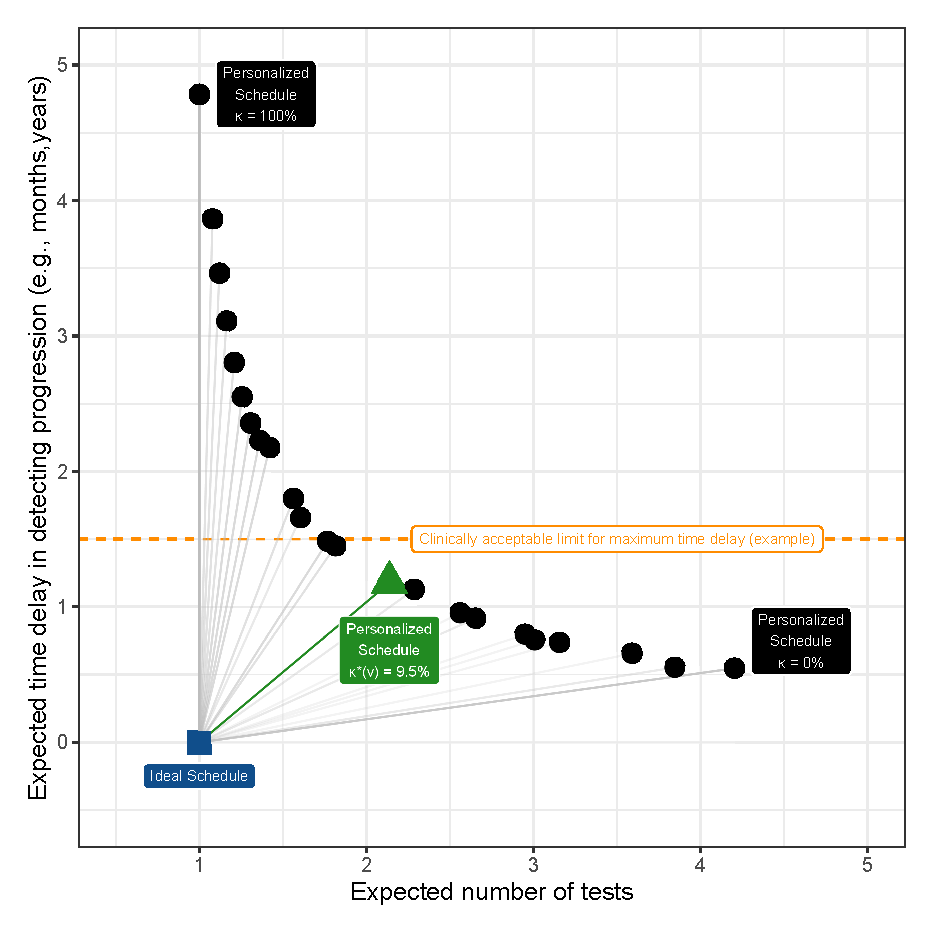
\includegraphics{images/kappa_choice_102.eps}}
\caption{\textbf{Automatic choice of risk threshold $0 \leq \kappa^* \leq 1$ using~(\ref{eq:kappa_choice})}. The ideal schedule of tests at point (1,0) is shown as a blue square. It plans exactly one invasive test at the true time of progression $T^*_j$ of a patient and hence leads to a zero time delay in detecting progression. Personalized schedules based on a grid of thresholds chosen between $0 \leq \kappa^* \leq 1$ are shown with black circles. Higher thresholds lead to fewer tests, but also higher expected time delay. We propose to choose the personalized schedule based on $\kappa^*(v)=9.5\%$ threshold (green triangle). This is because it has the least Euclidean distance (shown with a green line) to the ideal schedule. It is also possible to find the least distance under a certain clinically acceptable limit on time delay (orange dashed line), or number of tests.}
\label{fig:kappa_choice}
\end{figure}
% !TEX root =  ../main_manuscript.tex 
\section{Demonstration of Personalized Schedules}
\label{sec:results}
To demonstrate the application of personalized schedules on real patients, we return to the prostate cancer active surveillance dataset, PRIAS, described in Section~\ref{sec:introduction}. The current PRIAS protocol for biopsies is fixed biopsies at year one, four, seven, and ten of follow-up, and every five years after that. Additional annual biopsies are scheduled if a patient's PSA doubling-time~\citep{bokhorst2015compliance} is high. The PSA is measured as per a fixed schedule, quarterly for the first two years, and semi-annually after that. The DRE is also measured semi-annually. The dataset is summarized in Web-Appendix~B.

The clinical data that we intend to use consists of longitudinal PSA (continuous: ng/mL) and DRE (binary: tumor palpable or not) measurements, patient age at baseline, history of biopsies, and interval-censored times of cancer progression. The event of interest is cancer progression. We aim to use the accumulated clinical data to build a joint model that can be utilized for creating personalized biopsy schedules in future PRIAS patients.

\subsection{Fitting the Joint Model to the PRIAS Dataset}
We fit a joint model with $\log_2(\mbox{PSA} + 1)$ transformed PSA~\citep{lin2000latent,pearson1994mixed}, and DRE as longitudinal outcomes, and cancer progression as the event (Web-Appendix~B.3 for exact specification). For PSA, we utilize a linear mixed-effects sub-model wherein PSA profiles are modeled non-linearly over follow-up using B-splines~\citep{de1978practical}. For DRE, we utilize a logistic mixed-effects sub-model. To link the longitudinal sub-models for the PSA and DRE with the relative-risk sub-model for cancer progression, we include three features of the longitudinal outcomes in the relative-risk sub-model. Specifically, the hazard of cancer progression at time $t$ depends on the fitted instantaneous $\log_2(\mbox{PSA} + 1)$ value at time $t$, the estimated instantaneous $\log_2(\mbox{PSA} + 1)$ velocity at $t$, and fitted log-odds of having a DRE indicating a palpable tumor at $t$. We estimated the parameters of our model under the Bayesian framework using the R package \textbf{JMbayes}~\citep{rizopoulosJMbayes}.  

The follow-up period of PRIAS is currently limited. Hence, our joint model is able to predict the cumulative-risk of progression only until the year ten of follow-up. The cumulative-risk of progression at year ten in PRIAS is 50\% (Web-Figure~1). We found that the strongest predictor for progression in our model is $\log_2(\mbox{PSA} + 1)$ velocity. Specifically, for an increase in fitted $\log_2(\mbox{PSA} + 1)$ velocity from -0.03 to 0.15 the adjusted hazard ratio of progression was 1.6 (95\%CI: 1.45--1.78). Detailed parameter estimates are in Web-Appendix~B.4. Since personalized schedules are risk-based, their overall performance is dependent on the predictive accuracy of the fitted model. In this regard, the PRIAS based model's time-dependent area under the receiver operating characteristic curve~\citep{rizopoulos2011dynamic} was moderate (between 0.61 and 0.68) and time-dependent mean absolute prediction error~\citep{rizopoulos2011dynamic} was moderate to large (between 0.08 and 0.24) over follow-up (Web-Appendix~B.6).

\subsection{Personalized Schedules for a Demonstration Patient}
We utilized the joint model fitted to the PRIAS dataset to schedule biopsies in a real PRIAS patient (Figure~\ref{fig:demo_schedule}), starting from his current visit at year five, until year ten of follow-up. This patient has not progressed until year 3.5, and hence even if he incurs a delay in detecting progression of up to three years, it may not lead to adverse outcomes~\citep{carvalho}. Also, since his cumulative-risk of progression at year ten is only 16.5\%, he is likely to progress slowly. Consequently, few biopsies are planned by risk-based personalized schedules (Panel~B, Figure~\ref{fig:demo_schedule}). Even if this patient progresses before year ten of follow-up and opts for personalized schedules, not only will he undergo fewer biopsies than annual schedule (Panel~C, Figure~\ref{fig:demo_schedule}), but his expected delay in detecting progression is also under the aforementioned limit of three years (Panel~D, Figure~\ref{fig:demo_schedule}).
\begin{figure}
\centerline{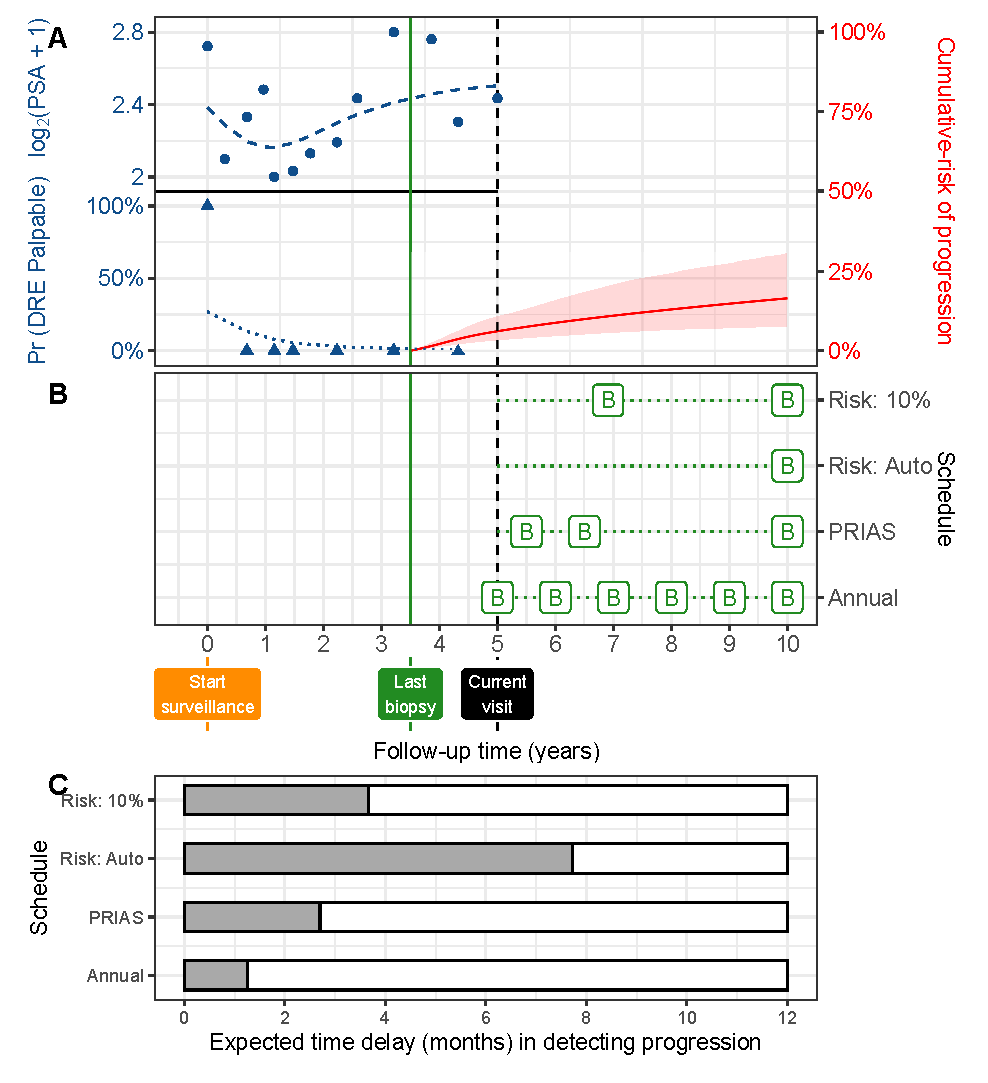
\includegraphics{images/demo_schedule.eps}}
\caption{\textbf{Demonstration of personalized schedules for a real PRIAS patient:} In \textbf{Panel~A}: Time of last negative biopsy is year 3.5 (vertical green solid line). Longitudinal data is repeated DRE (blue triangles) and PSA measurements (blue circles). The current visit is year five (vertical black dashed line). The estimated cumulative-risk profile is shown with a solid red line (95\% credible interval is shaded). It is 16.5\% at year ten (horizon). In \textbf{Panel~B}, we visualize different biopsy schedules, with a `B' indicating a biopsy. \textbf{$\kappa^*=10\%$} and \textbf{$\kappa^*(v)$} are personalized biopsy schedules using a fixed risk threshold of 10\%, and automatically chosen threshold~(\ref{eq:kappa_choice}), respectively. PRIAS and Annual denote the PRIAS biopsy schedule (paragraph~2 of Section~\ref{sec:results}) and annual biopsy schedule. \textbf{Panel~C,D}: For all schedules we calculate the expected number of tests and expected time delay in detecting progression if the patient progresses before year ten. Since a recommended minimum gap of one year is maintained between biopsies, maximum possible number of tests are six.  A delay in detecting progression of up to three years may not lead to adverse outcomes~\citep{carvalho}. }\label{fig:demo_schedule}
\end{figure}
% !TEX root =  ../main_manuscript.tex 
\section{Simulation Study}
\label{sec: simulation_study}
In Section \ref{subsec : demo_prias_pers_schedule} we demonstrated that the personalized schedules, schedule future biopsies according to the historical data of each patient. However, we could not perform a full-scale comparison between personalized and PRIAS schedules, because the true time of GR was not known for the PRIAS patients. To this end, we conducted a simulation study comparing personalized schedules with PRIAS and annual schedule, whose details are presented next.

\subsection{Simulation Setup}
\label{subsec : simulation_setup}
The population of AS patients in this simulation study is assumed to have the same entrance criteria as that of PRIAS. The PSA and hazard of GR for these patients follow a joint model of the form postulated in Section \ref{subsec : jm_fit_prias}, with parameters equal to the posterior mean of parameters estimated from the joint model fitted to the PRIAS dataset (see Web Appendix C). Furthermore, we also intend to test the efficacy of different schedules for a population which has patients with both faster as well as slowly-progressing PCa. The rate of progression is not only manifested via PSA profiles but also via the baseline hazard. We assume that there are three equal sized subgroups $G_1$, $G_2$ and $G_3$ of patients in the population, each with a baseline hazard from a Weibull distribution, with the following shape and scale parameters $(k, \lambda$): $(1.5, 4)$, $(3, 5)$ and $(4.5, 6)$ for $G_1, G_2$ and $G_3$, respectively. The effect of these parameters is that the mean GR time is lowest in $G_1$ (fast PCa progression) and highest in $G_3$ (slow PCa progression).

From this population, we have sampled 500 datasets with 1000 patients each. We generate a true GR time for each of the patients, and then sample a set of PSA measurements at the same time points as given in PRIAS protocol (see Web Appendix C). We then split the dataset into a training (750 patients) and a test (250 patients) part, and generate a random and non-informative censoring time for the training patients. We next fit a joint model of the specification given in (\ref{eq : long_model_prias}) and (\ref{eq : hazard_prias}) to each of the 500 training datasets and obtain MCMC samples from the 500 sets of the posterior distribution of the parameters. Using these fitted joint models, we obtain the posterior predictive distribution of time of GR for each of the $500 \times 250$ test patients. This distribution is further used to create personalized biopsy schedules for the test patients. For every test patient we conduct hypothetical biopsies using the following six types of schedules (abbreviated names in parenthesis): personalized schedules based on expected time of GR (Exp. GR time) and median time of GR (Med. GR time), personalized schedules based on dynamic risk of GR (Dyn. risk GR), a hybrid approach between median time of GR and dynamic risk of GR (Hybrid), PRIAS schedule and the annual schedule. The biopsies are conducted as per the algorithm in Figure \ref{fig : sched_algorithm}. 

To compare the aforementioned schedules we require estimates of the various measures of efficacy described in Section \ref{sec : choosing_schedule}. To this end, for schedule $S$, we compute pooled estimates of mean offset $E(O^S_j)$ and variance of offset $\mbox{var}(O^S_j)$, as below (estimates for $N^S_j$ are similar):
\begin{align*}
\widehat{E(O^S_j)} &= \frac{\sum_{k=1}^{500} n_k \widehat{E(O^S_k)}}{\sum_{k=1}^{500} n_k}, \\
\widehat{\mbox{var}(O^S_j)} &= \frac{\sum_{k=1}^{500} (n_k - 1) \widehat{\mbox{var}(O^S_k)}}{\sum_{k=1}^{500} (n_k-1)}, 
\end{align*}
where $n_k$ denotes the number of test patients, $\widehat{E(O^S_k)} = {\sum_{l=1}^{n_k}O^S_{kl}}/{n_k}$ is the estimated mean and $\widehat{\mbox{var}(O^S_k)} = {\sum_{l=1}^{n_k}\big\{O^S_{kl} - \widehat{E(O^S_k)}\big\}^2}/(n_k-1)$ is the estimated variance of the offset for the $k$-th simulation. The offset for the $l$-th test patient of the $k$-th dataset is denoted by $O^S_{kl}$.

\subsection{Results}
The pooled estimates of the aforementioned measures are summarized in Table \ref{table : sim_study_pooled_estimates}. In addition, estimated values of $E(O^S_j)$ are plotted against $E(N^S_j)$ in Figure \ref{fig : meanNbVsOffset}. The figure shows that across the schedules there is an inverse relationship between number $E(O^S_j)$ and $E(N^S_j)$. For example, the annual schedule conducts on average 5.2 biopsies to detect GR, which is the highest among all schedules. However, it has the least average offset of 6 months as well. On the other hand, the schedule based on expected time of GR conducts only 1.9 biopsies on average to detect GR, the least among all schedules, but it also has the highest average offset of 15 months (similar for median time of GR). Since the annual schedule attempts to contain the offset within a year it has the least $\mbox{SD}(O^S_j) = \sqrt{\mbox{var}(O^S_j)}$. However to achieve this, it conducts a wide range of number of biopsies from patient to patient, i.e., highest $\mbox{SD}(N^S_j) = \sqrt{\mbox{var}(N^S_j)}$. In this regard, schedules based on expected and median time of GR perform the opposite of annual schedule.

\begin{figure}
\centerline{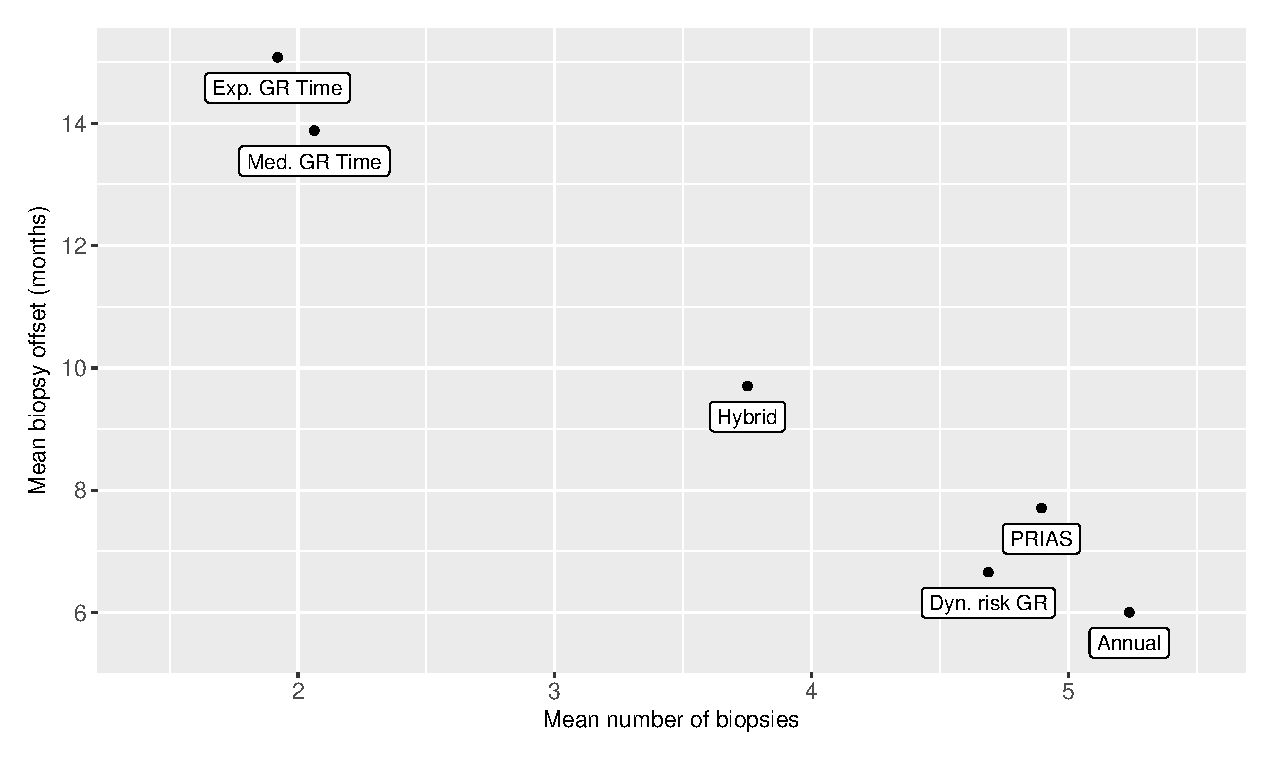
\includegraphics[width=\columnwidth]{images/sim_study/meanNbVsOffset_all.eps}}
\caption{Estimated mean number of biopsies and mean offset (months) for various schedules, obtained from the simulation study with 500 simulated datasets.}
\label{fig : meanNbVsOffset}
\end{figure}

%124781 = 41484 + 41423 + 41874
\begin{table}
\caption{Estimated mean and standard deviation of the number of biopsies $N^S_j$ and offset $O^S_j$ (months) for various schedules, obtained from the simulation study with 500 simulated datasets.}
\label{table : sim_study_pooled_estimates}
\begin{tabular}{lrrrr}
\Hline
\multicolumn{5}{c}{a) All hypothetical subgroups}\\
\hline
Schedule          & $E(N^S_j)$ & $E(O^S_j)$ & ${\mbox{SD}(N^S_j)}$ & ${\mbox{SD}(O^S_j)}$ \\
\hline
Annual         & 5.24            & 6.01                & 2.53          & 3.46              \\
PRIAS          & 4.90            & 7.71                & 2.36          & 6.31\\
Dyn. risk GR       & 4.69            & 6.66                & 2.19           & 4.38              \\
Hybrid       & 3.75            & 9.70                & 1.71          & 7.25              \\
Med. GR time & 2.06            & 13.88               & 1.41          & 11.80              \\
Exp. GR time & 1.92            & 15.08               & 1.19          & 12.11             \\
\hline
\multicolumn{5}{c}{b) Hypothetical subgroup $G_1$}\\
\hline
Schedule        & $E(N^S_j)$ & $E(O^S_j)$ & ${\mbox{SD}(N^S_j)}$ & ${\mbox{SD}(O^S_j)}$ \\
\hline
Annual         & 4.32            & 6.02                & 3.13          & 3.44              \\
PRIAS          & 4.07            & 7.44                & 2.88          & 6.11    \\
Dyn. risk GR       & 3.85            & 6.75                & 2.69          & 4.44              \\
Hybrid       & 3.25            & 10.25               & 2.16          & 8.07              \\
Med. GR time & 1.84            & 20.66               & 1.76          & 14.62             \\
Exp. GR time & 1.72            & 21.65               & 1.47          & 14.75             \\
\hline      
\multicolumn{5}{c}{c) Hypothetical subgroup $G_2$}\\
\hline
Schedule        & $E(N^S_j)$ & $E(O^S_j)$ & ${\mbox{SD}(N^S_j)}$ & ${\mbox{SD}(O^S_j)}$ \\
\hline
Annual         & 5.18            & 5.98                & 2.13          & 3.47              \\
PRIAS          & 4.85            & 7.70                & 2.00          & 6.29        \\
Dyn. risk GR       & 4.63            & 6.66                & 1.82          & 4.37              \\
Hybrid       & 3.68            & 10.32                & 1.37          & 7.45              \\
Med. GR time & 1.89             & 12.33               & 1.16          & 9.44              \\
Exp. GR time & 1.77            & 13.54               & 0.98          & 9.83              \\
\hline      
\multicolumn{5}{c}{d) Hypothetical subgroup $G_3$}\\
\hline
Schedule        & $E(N^S_j)$ & $E(O^S_j)$ & ${\mbox{SD}(N^S_j)}$ & ${\mbox{SD}(O^S_j)}$ \\
\hline
Annual         & 6.20             & 6.02                & 1.76          & 3.46              \\
PRIAS          & 5.76             & 7.98                & 1.71         & 6.51        \\
Dyn. risk GR       & 5.58            & 6.58                & 1.56          & 4.33              \\
Hybrid       & 4.32            & 8.55                & 1.26          & 5.91              \\
Med. GR time & 2.45            & 8.70                & 1.15          & 6.32              \\
Exp. GR time & 2.27            & 10.09               & 0.99          & 7.47              \\
\hline     
\end{tabular}
\end{table}

The PRIAS schedule conducts only 0.3 biopsies less than the annual schedule, but with a higher $\mbox{SD}(O^S_j)$, early detection is not always guaranteed. In comparison, the dynamic risk of GR based schedule performs slightly better than the PRIAS schedule in all four criteria. The hybrid approach combines the benefits of methods with low $E(N^S_j)$ and $\mbox{SD}(N^S_j)$, and methods with low $E(O^S_j)$ and $\mbox{SD}(O^S_j)$. It conducts 1.5 biopsies less than the annual schedule on average and with a $E(O^S_j)$ of 9.7 months it detects GR within a year since its occurrence. Moreover, it has both $\mbox{SD}(N^S_j)$ and $\mbox{SD}(O^S_j)$ comparable to PRIAS.

The performance of each schedule differs for the three subgroups $G_1, G_2$ and $G_3$. The annual schedule remains the most consistent across subgroups in terms of the offset, but it conducts 2 extra biopsies for the subgroup $G_3$ (slowly-progressing PCa) than $G_1$ (faster-progressing PCa). The performance of schedule based on expected time of GR is the most consistent in terms of the number of biopsies but it detects GR a year later on average in subgroup $G_1$ than $G_3$. For the dynamic risk of GR based schedule and the hybrid schedule, the dynamics are similar to that of the annual schedule. Unlike the latter two schedules, the PRIAS schedule not only conducts more biopsies in $G_3$ than $G_1$ but also detects GR later in $G_3$ than $G_1$.

\begin{figure}[!htb]
\centerline{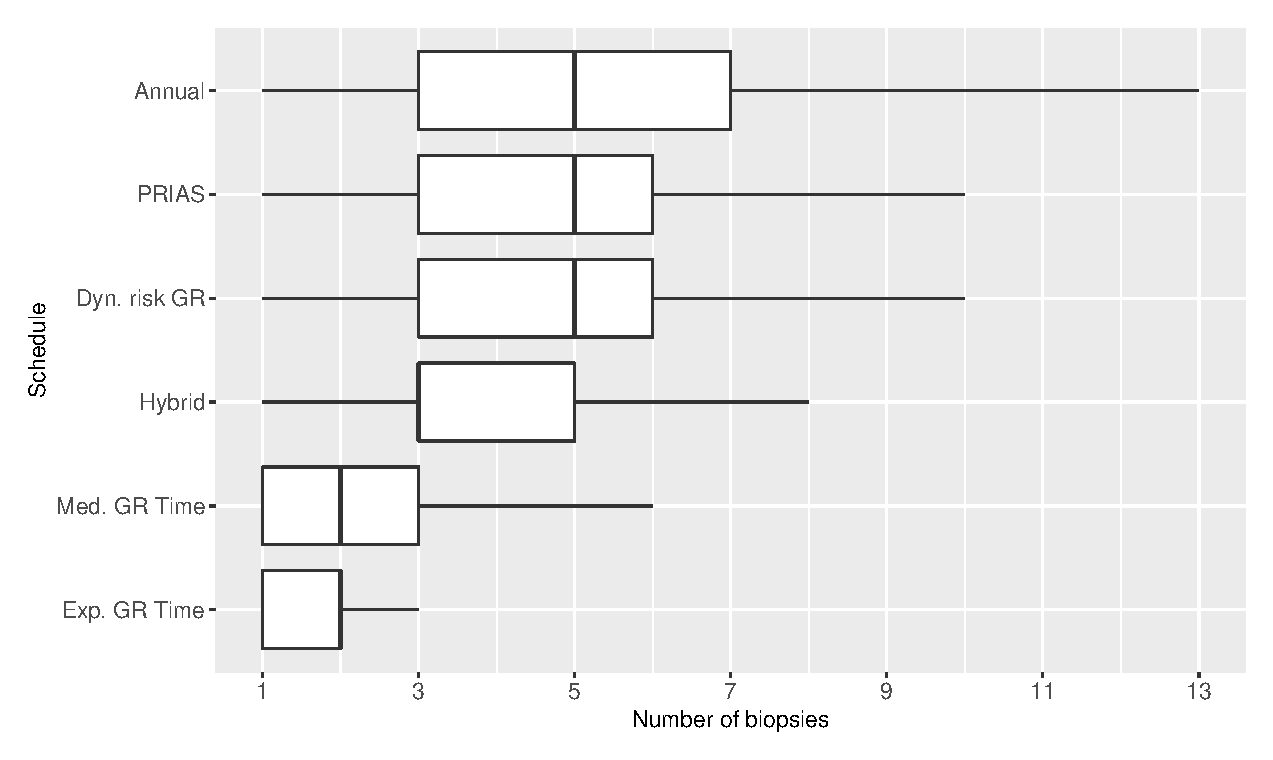
\includegraphics[width=\columnwidth]{images/sim_study/nbBoxPlot_all.eps}}
\caption{Boxplot showing variation in number of biopsies conducted by various schedules, obtained from the simulation study with 500 simulated datasets.}
\label{fig : nbBoxPlot_all}
\end{figure}

\begin{figure}[!htb]
\centerline{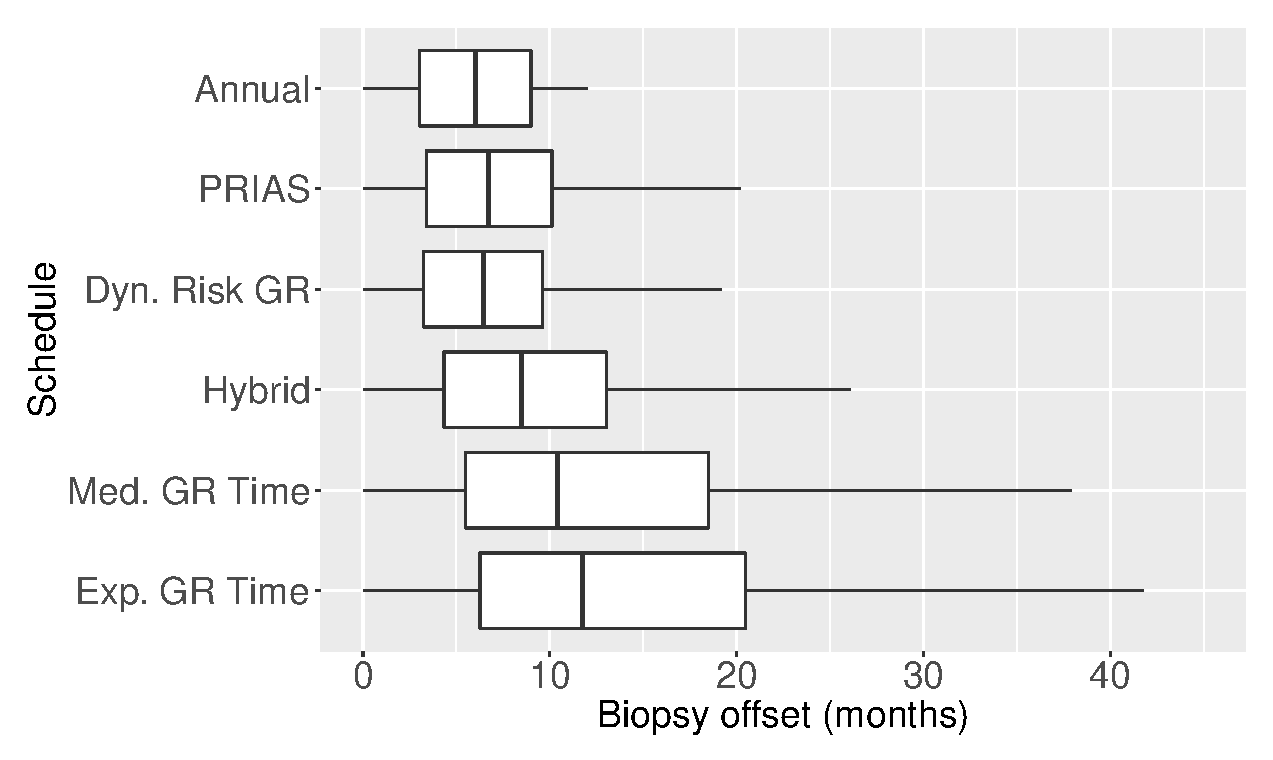
\includegraphics[width=\columnwidth]{images/sim_study/offsetBoxPlot_all.eps}}
\caption{Boxplot showing variation in biopsy offset (months) for various schedules, obtained from the simulation study with 500 simulated datasets.}
\label{fig : offsetBoxPlot_all}
\end{figure}

The choice of a suitable schedule using (\ref{eq : loss_func_sim_study_generic}) depends on the chosen measure for evaluation of schedules. In this regard, the schedules we compared either have high $\mbox{SD}(O^S_j)$ and low $\mbox{SD}(N^S_j)$, or vice versa (Table \ref{table : sim_study_pooled_estimates}). Thus, applying a cutoff on $E(O^S_j)$ when $\mbox{SD}(O^S_j)$ is high may not be as fruitful (same for $N^S_j$) as applying a cutoff on $\mbox{SD}(O^S_j)$ or quantile(s) of $O^S_j$. For example, the schedule based on the dynamic risk of GR is suitable if on average the least number of biopsies are to be conducted to detect GR, while simultaneously making sure that at least 90\% of the patients have an average offset less than one year.

% !TEX root =  ../main_manuscript.tex 
\section{Discussion}
\label{sec:discussion}
In this paper, we presented a methodology to create personalized schedules for burdensome diagnostic \textit{tests} utilized to detect disease \textit{progression} in early-stage chronic non-communicable disease \textit{surveillance}. For this purpose, we utilized joint models for time-to-event and longitudinal data. Our approach first combines a patient's clinical data (e.g., longitudinal biomarkers) and previous invasive test results to estimate patient-specific cumulative-risk of disease progression over their current and future follow-up visits. We then plan future invasive tests whenever this cumulative-risk of progression is predicted to be above a certain threshold. We select the risk threshold automatically in a personalized manner, by optimizing a utility function of the patient-specific consequences of choosing a particular risk threshold based schedule. These consequences are, namely, the number of invasive tests (burden) planned in a schedule, and the expected time delay in detection of progression (shorter is beneficial) if the patient progresses. Last, we calculate this expected time delay in a personalized manner for both personalized and fixed schedules to assist patients/doctors in making a more informed decision of choosing a test schedule.

Using joint models gives us certain advantages. First, since joint models employ random-effects, the corresponding risk-based schedules are inherently personalized. Second, to predict this patient-specific risk of progression, joint models utilize all observed longitudinal measurements of a patient. Also, the continuous longitudinal outcomes are not discretized, which is commonly a case in Markov Decision Process and flowchart-based test schedules. Third, personalized schedules update automatically with more patient data over follow-up. Fourth, we calculated the expected number of tests (burden) and expected time delay in detecting progression (shorter is beneficial) in a patient-specific manner. Using our methodology, these can be calculated for both personalized and fixed schedules. Thus, patients/doctors can compare risk-based and fixed schedules and choose one according to their preferences for the expected burden-benefit ratio. Last, although this work concerns invasive test schedules in disease surveillance, the methodology is generic for use under a screening setting as well.

Personalized schedules that we proposed require a risk threshold. We optimized the threshold choice using a generic utility function based on the expected number of biopsies and time delay in detecting progression. We used only these two measures because they are easy to interpret but simultaneously critical for deciding the timing of invasive tests. Also, the time delay in detecting progression should manifest the window of opportunity for curative treatment and additional benefits of observing progression early. Practitioners may extend/modify this utility function by adding to/replacing time delay with commonly used decision-theoretic measures such as quality-adjusted life-years/expectancy (QALY/QALE).

We evaluated personalized schedules in a full cohort via a realistic simulation of a randomized clinical trial for prostate cancer surveillance patients. We observed that personalized schedules reduced many unnecessary biopsies for non-progressing patients compared to the widely used annual schedule. This happened at the cost of simultaneously having a slightly more time delay in detecting progression. Although, this delay should still be safe because it was almost equal to the delay of the world's largest prostate cancer active surveillance program PRIAS's schedule. The simulation study results are by no means the performance-limit of the personalized schedules. Instead, models with higher predictive accuracy and discrimination capacity than the PRIAS based model may lead to an even better balance between the number of tests and the time delay in detecting progression.

There are certain limitations to this work. First, in practice, most cohorts have a limited study period. Hence, the cumulative-risk profiles of patients and resulting personalized schedules can only be created up to the maximum study period. For this problem, the risk prediction model should be updated with more follow-up data over time. The proposed joint model assumed all events other than progression to be non-informative censoring. Alternative models that account for competing risks may lead to better results as they estimate absolute and not the cause-specific risk of progression. Upgrading is susceptible to inter-observer variation and sampling error. Although models that account for these two issues~\citep{balasubramanian2003estimation,coley2017prediction} will provide better risk estimates, the methodology for obtained personalized schedules can remain the same.

%  The \backmatter command formats the subsequent headings so that they
%  are in the journal style.  Please keep this command in your document
%  in this position, right after the final section of the main part of 
%  the paper and right before the Acknowledgements, Supporting Information (Supplementary %  Materials),   and References sections. 

\backmatter

%  This section is optional.  Here is where you will want to cite
%  grants, people who helped with the paper, etc.  But keep it short!

\section*{Acknowledgments}
The first and last authors would like to acknowledge support by Nederlandse Organisatie voor Wetenschappelijk Onderzoek (the national research council of the Netherlands) VIDI grant nr. 016.146.301, and Erasmus University Medical Center funding. Part of this work was carried out on the Dutch national e-infrastructure with the support of SURF Cooperative. The authors also thank the Erasmus University Medical Center's Cancer Computational Biology Center for giving access to their IT-infrastructure and software that was used for the computations and data analysis in this study.

This work was supported by the Movember Foundation. The funder did not play any role in the study design, collection, analysis or interpretation of data, or in the drafting of this paper.

\section*{Data Availability}
This work utilized results from a statistical model we previously fitted to the PRIAS dataset~\citep{tomer2019personalized}. The PRIAS database is not openly accessible. However, access to the database can be requested on the basis of a study proposal approved by the PRIAS steering committee. The website of the PRIAS program is \textcolor{blue}{www.prias-project.org}. For sake of completeness and reproducibility of results, we have presented the PRIAS based model's definition and parameter estimates in Web-Appendix~B. The data of the demonstration patient in Figure~\ref{fig:demo_schedule} is provided in Web-Appendix~B.

\section*{Supporting Information}
Web Appendices referenced in this paper are available in the file titled `supplementary.pdf'.

%  Here, we create the bibliographic entries manually, following the
%  journal style.  If you use this method or use natbib, PLEASE PAY
%  CAREFUL ATTENTION TO THE BIBLIOGRAPHIC STYLE IN A RECENT ISSUE OF
%  THE JOURNAL AND FOLLOW IT!  Failure to follow stylistic conventions
%  just lengthens the time spend copyediting your paper and hence its
%  position in the publication queue should it be accepted.

%  We greatly prefer that you incorporate the references for your
%  article into the body of the article as we have done here 
%  (you can use natbib or not as you choose) than use BiBTeX,
%  so that your article is self-contained in one file.
%  If you do use BiBTeX, please use the .bst file that comes with 
%  the distribution.  In this case, replace the thebibliography
%  environment below by 
%
%  \bibliographystyle{biom} 
% \bibliography{mybibilo.bib}

\bibliographystyle{biom} 
\bibliography{bibliography}

%  If your paper refers to supporting web material, then you MUST
%  include this section!!  See Instructions for Authors at the journal
%  website http://www.biometrics.tibs.org
\end{document}
